\chapter{Afgeleide klassen en objecten in C++} \label{chap:inh}

Bij deze opdracht kijken we hoe bij OO componenten Overerving en Polymorfisme kunnen testen met een debugger.

Deze opdracht bestaat uit de deelopdrachten A en B. Er moeten 6 screenshots gemaakt worden die op Brightspace moeten worden geüpload. Alle deelopdrachten moet je laten aftekenen door de docent.

Er zijn diverse soorten LED's, zoals in Figuur \ref{fig:LEDs} te zien zijn. Deze zijn:
\begin{itemize}
	\item SingleLed: deze LED's hebben 1 kleur, twee pootjes en worden aan 1 poort op de RockPi aangesloten, zoals de rode, oranje en groene LED. Een voorbeeld wordt weergegeven in Figuur \ref{fig:singleLed}
	\item DualLed: deze LEDs hebben 2 kleuren; rood en groen, drie pootjes en worden aan 2 poorten (1 per kleur) aan de RockPi verbonden. Een voorbeeld wordt weergegeven in Figuur \ref{fig:dualLed}
	\item RGB Led: deze LED's hebben de kleuren rood, groen en blauw in 1 behuizing en hebben vier pootjes, waarvan 3 worden aangesloten op de poorten (1 per kleur) van de RockPi. De LED met de witte kleur op het practicumbord is een RGB LED. Een voorbeeld van een RGB LED wordt weergegeven in Figuur \ref{fig:rgbLed}
\end{itemize}

\begin{figure}[h!]
	\centering
	\begin{subfigure}[b]{0.3\textwidth}
		\centering
		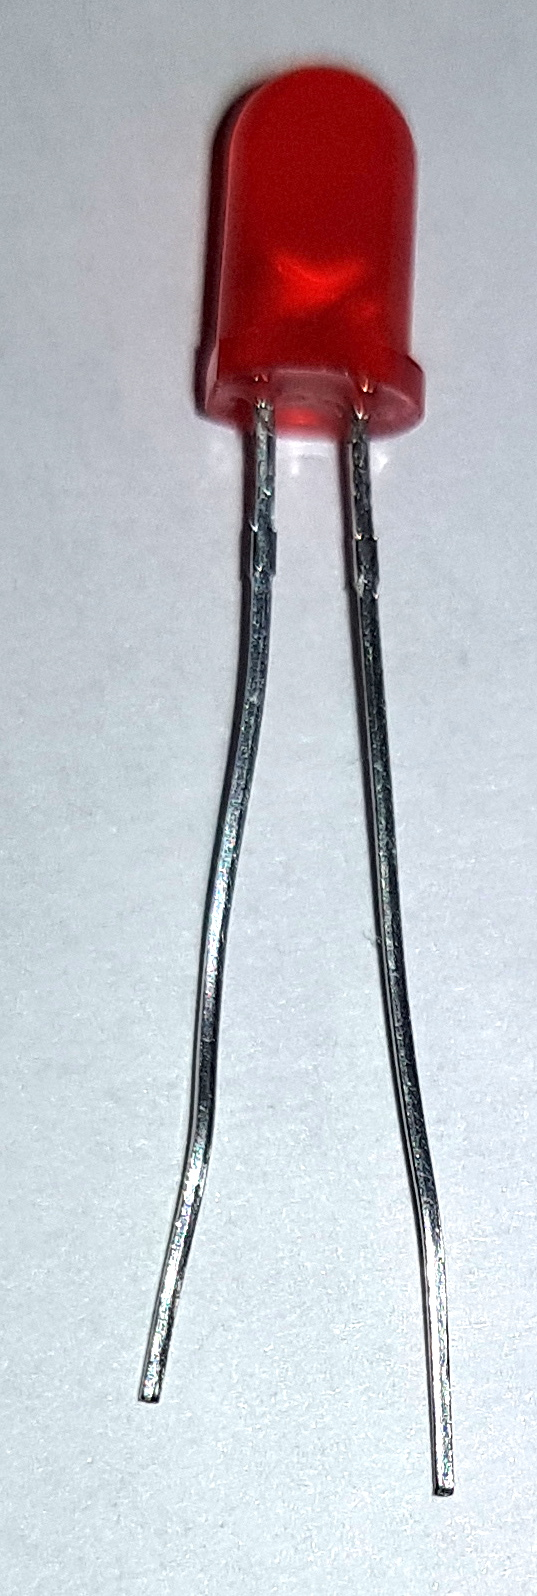
\includegraphics[width=0.7\textwidth,height=3.5cm]{figuren/singleled}
		\caption{een single LED}
		\label{fig:singleLed}
	\end{subfigure}
	\hfill
	\begin{subfigure}[b]{0.3\textwidth}
		\centering
		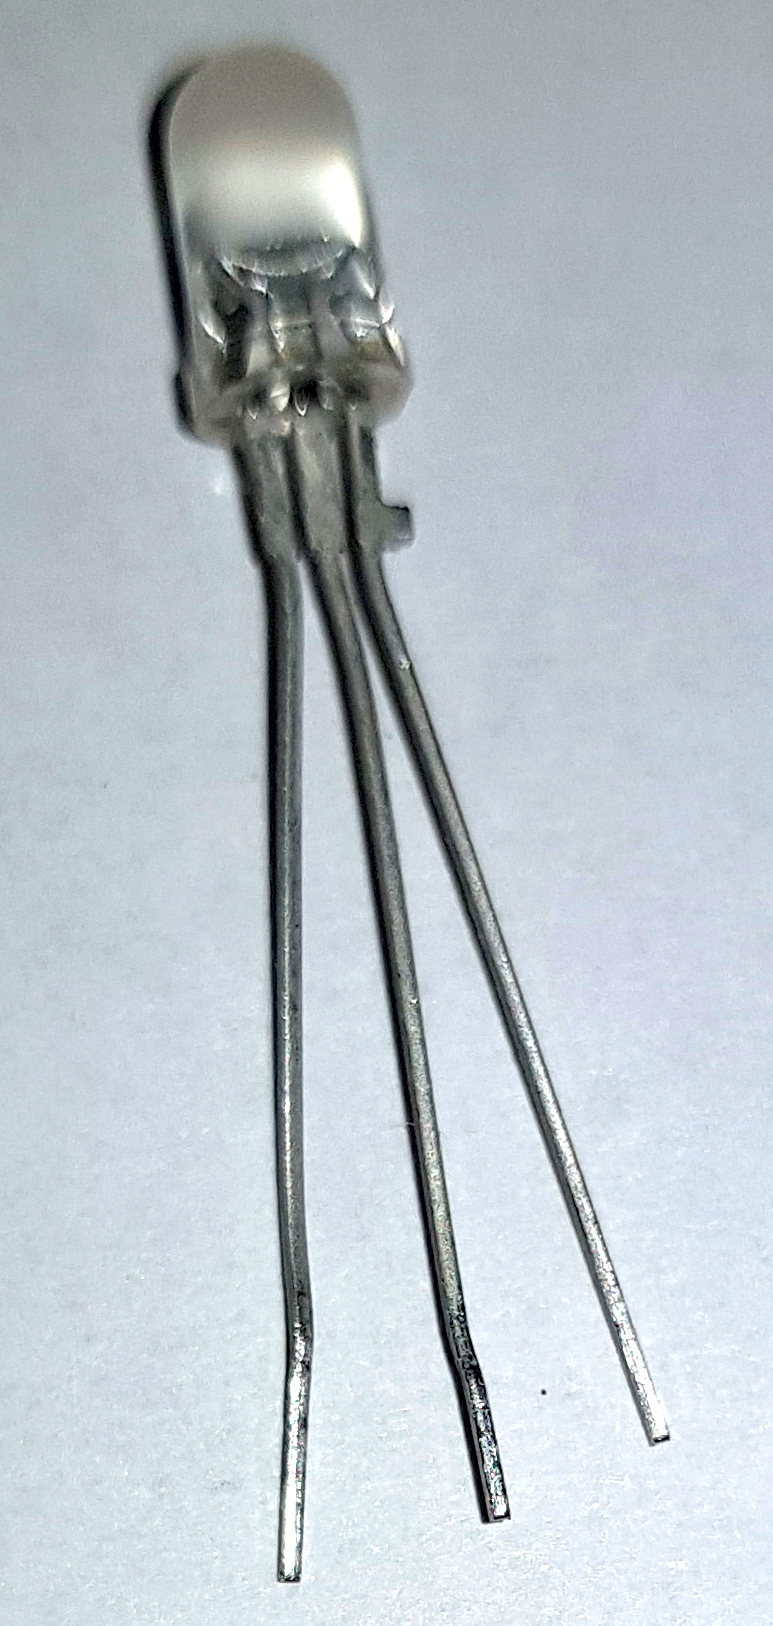
\includegraphics[width=0.7\textwidth,height=3.5cm]{figuren/dualled}
		\caption{een dual LED}
		\label{fig:dualLed}
	\end{subfigure}
	\hfill
	\begin{subfigure}[b]{0.3\textwidth}
		\centering
		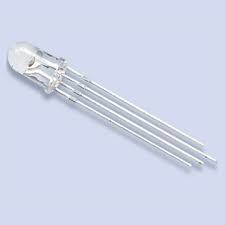
\includegraphics[width=0.9\textwidth,height=3.5cm]{figuren/rgbled}
		\caption{een RGB LED}
		\label{fig:rgbLed}
	\end{subfigure}
	\caption{Verschillende type LEDs}
	\label{fig:LEDs}
\end{figure}

De analist die de eisen voor de controller-software voor de LED controllers opstelt, heeft bedacht dat het in de toekomst mogelijk moet kunnen zijn om nieuwe LED types toe te voegen, bijvoorbeeld 3 kleuren LEDS. De controller software moet dus zo veel mogelijk onafhankelijk van het concrete LED type gemaakt worden. In Figuur \ref{fig:klassLed} wordt de UML weergave getoond van zowel de SingleLed als van de RGBLed
\begin{figure}[h!]
	\captionsetup{justification=centering}
	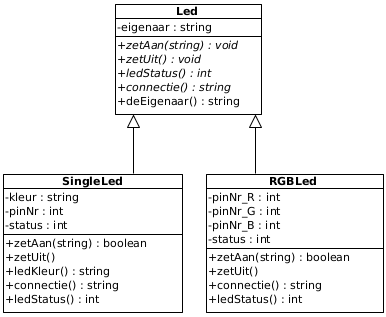
\includegraphics[width=0.6 \linewidth]{figuren/rgbKlasse}
	\centering
	\caption{De afgeleide klassen singleLed en RGBLed .}
	\label{fig:klasAfg}
\end{figure}
\newpage
De werking is als volgt.

\begin{itemize}
	\item Een LED wordt aangezet door de methode bool zetAan(string k); waarbij de parameter de kleur is die aangezet moet worden.
	\begin{itemize}
		\item Wordt bij een groene LED ''groen''  meegegeven, wordt de LED aangezet en true geretourneerd.
		\item Wordt bij een groene LED ''rood'' meegegeven, wordt de LED niet aangezet en wordt false geretourneerd.
	\end{itemize}
\item Een LED wordt uitgezet door de methode \texttt{void zetUit();} Dit houdt in dat bij een RGBLed alle kleuren uitgezet worden.
\item De methode \texttt{string connectie();} geeft het gpioNummer van het aangesloten platform mee terug. In het geval van de RGBLed wordt een string mee teruggegeven met alle drie de gpioNummers gescheiden door een spatie.
\item Doordat de status van LED's verschillend zijn (een singleLed kan alleen aan en uit terwijl bij de RGBLed kleur 1, kleur 2, kleur 3 of een combinatie van kleuren kan aan- en uitgaan), heeft elke afgeleide LED een eigen status.
\item Omdat bij een RGBLed al bekend is wat de kleuren zijn (Rood, Groen en Blauw), hoeft de kleur van de LED niet opgevraagd te worden. In tegenstelling tot een singleLed die maar \'{e}\'{e}n kleur heeft, dit kunnen overigens verschillende kleuren zijn.
\end{itemize}

%\paragraph{Opdracht} 
\newpage
\section{De Klasse SingleLed} \label{sec:singleLed}

Zoals in Figuur \ref{fig:klasAfg} wordt aangegeven is de singleLed een speciale vorm van Led. \\Dit is ook terug te zien in de code, zoals Listing \ref{lst:singleLedH} laat zien.

\noindent\begin{minipage}{.45\textwidth}
\begin{lstlisting}[caption=LED declaratie file(.h),frame=tlrb,label={lst:ledBaseH}]{Name}
class Led
{
	public:
	/*
		Implementeer hier 
	de constructor(s) 
	en de methoden
	*/
	
	private:
       string eigenaar;
};
\end{lstlisting}
\end{minipage}\hfill
\begin{minipage}{.45\textwidth}
\begin{lstlisting}[caption=SingleLed declaratie file(.h),frame=tlrb,label={lst:singleLedH}]{Name}
class SingleLed : public Led
{
	public:
	/*
	Implementeer hier 
	de constructor(s) 
	en de methoden
	*/

	private:
        string kleur;
	    int pinNr;
	    int status;
};
\end{lstlisting}
\end{minipage}
\paragraph{Opdracht} 
\begin{enumerate}[label=(\alph*)]
\item Clone de code van git: \\
{\small \texttt{git clone } \verb|--|\texttt{branch opdracht31 https://github.com/JohnVi-hhs/oop.git}}
\item
Implementeer de klasse Led en SingleLed (zowel de .h als de .cpp file ).
Hierbij kan inspiratie opgedaan worden bij de klassen Hond, Tekkel en SintBernard uit het college en de bijbehorende code uit bijlage \ref{cpt:klHonden}. Run vervolgens de main code van Listing \ref{lst:mainSled}.\\~\\
TIP: in de code wordt gevraagd om de \texttt{int pinNr} als \texttt{string} af te drukken. Deze omzetting heet een cast, dit doe je met het commando \texttt{to\_string(pinNr)}
\newpage

\begin{lstlisting}[caption=main functie om de klasse SingleLed te testen. ,frame=trbl,firstnumber=1,numbers=left,label={lst:mainSled}]{Name}
#define GROENELED 132
#define GELELED 134
void LedInfo(Led& l) {
	cout<<"De eigenaar is:"<<l.deEigenaar()<<endl;
	cout<<"De Led is aangesloten op pinnen"<<l.connectie()<<endl;
	cout<<"De status van de Led is:"<<l.ledStatus()<<endl;
}

int main() {
	SingleLed led1(RODELED,"rood","Pietje Puk");
	SingleLed led2(GELELED,"geel");
	
	Led &lr1(led1);
	lr1.zetAan("rood");
	usleep(1000000);
	led2.zetAan("geel"); 
	usleep(1000000);
	led1.zetUit();
	usleep(1000000);
	
	LedInfo(led1);
	LedInfo(led2);
	LedInfo(lr1);
	
	led2.zetUit();
	return 0;
}

\end{lstlisting}

%De uitkomst van het programma wordt weergegeven op de volgende bladzijde.
%\newpage
De uitkomst van het programma is als volgt:\\
\texttt{De eigenaar is:Pietje Puk\\
De Led is aangesloten op pinnen135\\
De status van de Led is:0\\
De eigenaar is:Anoniem\\
De Led is aangesloten op pinnen134\\
De status van de Led is:1\\
De eigenaar is:Pietje Puk\\
De Led is aangesloten op pinnen135\\
De status van de Led is:0\\}

\newpage
\item 
\begin{itemize}
	\item Start de VNC viewer op met hierin de DDD debugger.
	\item Plaats een breakpoint op regel 21 van Listing \ref{lst:mainSled} ({\small \texttt{ LedInfo(led1) }}). \\ (Met \textbf{Alt + N} zet je de weergave van regelnummers aan.)
	\item Run het programma, de debugger zal stoppen op regel 21.
	\item Toon de objecten led1 en led2, zoals getoond in Figuur \ref{fig:DDDLed1_2}. 
	\begin{figure}[h!]
		\captionsetup{justification=centering}
%		\includegraphics[width=0.95 \linewidth]{figuren/DDDLed1Led2}
    	\includegraphics[width=0.95 \textwidth]{figuren/DDDLed1Led2}
		\centering
		\caption{De inhoud van objecten led1 en led2 .}
		\label{fig:DDDLed1_2}
	\end{figure}
	De tekst achter \texttt{\_vptr.led} kan verborgen worden door deze te selecteren en in de pull-down menu \textit{hide All} te kiezen. \\
	Verder is duidelijk te zien dat de base-klasse  \textbf{Led}, met het attribuut eigenaar, een onderdeel is van de afgeleide klasse \textbf{SingleLed}.
\end{itemize}

\item Maak een screenshot van beide objecten in de DDD debugger, uiteraard met je \textcolor{red}{\huge{eigen}} naam en plaatst deze met de \textbf{code} in je portfolio onder het hoofdstuk programmeren $\Longrightarrow$ subhoofdstuk \ref{sec:singleLed}. \\ 
Laat de opdracht aftekenen met de screenshots zichtbaar.

\end{enumerate}
\newpage
\section{De Klasse RGBLed} \label{sec:rgb}

Zoals te zien in het klassendiagram van Figuur \ref{fig:klasAfg} is de RGBLed ook een Led. Doordat bij een RGB LED de kleuren al bekend zijn, heeft deze klasse geen attribuut kleur. De klasse RGBLed heeft verder:
\begin{itemize}
	\item Drie aansluitingen op de RockPi, namelijk voor elke kleur 1. Deze aansluitingen zijn:
	\begin{itemize}
		\item 146 rood
		\item 149 groen
		\item 150 blauw
	\end{itemize}
    \item De methode connectie geeft de 3 aansluitnummers als een string mee terug, waarbij de spatie een onderscheid maakt tussen de pin-nummers.
    \item De status geeft aan welke kleur aan is. Dit wordt gedaan door elke kleur een bit toe te wijzen. De toewijzing is als volgt:
    \begin{itemize}
    	\item bit 0 rood
    	\item bit 1 groen
    	\item bit 2 blauw
    \end{itemize}

\end{itemize}
\newpage
 \paragraph{Opdracht}
 
\begin{enumerate}[label=(\alph*)]
	\item
	Implementeer de klasse RGBLed (zowel de .h als de .cpp file ) en run de main code van Listing \ref{lst:mainRGBLed}.
	
\begin{lstlisting}[caption=main functie om de klasse SingleLed te testen. ,frame=trbl,firstnumber=1,numbers=left,label={lst:mainRGBLed}]{Name}
void LedInfo(Led& l) {
	cout<<"De eigenaar is: "<<l.deEigenaar()<<endl;
	cout<<"De Led is aangesloten op pinnen: "<<l.connectie()<<endl;
	cout<<"De status van de Led is: "<<l.ledStatus()<<endl;
}
		
int main() {
   cout<<"Hi NSE, welkom bij opdracht 2"<<endl;

   RGBLed kleuren(RGB_R,RGB_G,RGB_B,"Pietje Puk");
   kleuren.zetAan("rood");
   usleep(1000000);
   kleuren.zetUit();
   kleuren.zetAan("groen");
   usleep(1000000);
   kleuren.zetUit();
   kleuren.zetAan("blauw");
   usleep(1000000);
   kleuren.zetAan("groen");
   usleep(1000000);
   kleuren.zetUit();
   kleuren.zetAan("rood");
   kleuren.zetAan("groen");
   usleep(1000000);
   kleuren.zetUit();
   kleuren.zetAan("rood");
   kleuren.zetAan("blauw");
   usleep(1000000);
   kleuren.zetAan("groen");
   usleep(1000000);
   LedInfo(kleuren);  
   kleuren.zetUit();

   cout<<"einde"<<endl;
}
		
\end{lstlisting}
 De uitkomst van het programma wordt weergegeven op de volgende bladzijde.
 \newpage
% De uitkomst van het programma:\\ \\
\texttt{Hi NSE, welkom bij opdracht 2\\
De eigenaar is: Pietje Puk\\
De Led is aangesloten op pinnen: 146 149 146\\
De status van de Led is: 7\\
einde\\ \\    
}
Plaats de code van de RGBLed (zowel de .h als de .cpp) file in je portfolio onder het hoofdstuk programmeren $\Longrightarrow$ subhoofdstuk \ref{sec:rgb}.

\item In deze opdracht worden zowel de SingleLed als de RGBLed gebruikt. Verder worden objecten van de klasse \textbf{SingleLed} en \textbf{RGBLed} in de DDD debugger getoond. Compileer de code van Listing \ref{lst:mainCombi} en run deze.
\begin{lstlisting}[caption=main functie om de klasse SingleLed te testen. ,frame=trbl,firstnumber=1,numbers=left,label={lst:mainCombi}]{Name}
void LedInfo(Led& l) {
	cout<<"De eigenaar is: "<<l.deEigenaar()<<endl;
	cout<<"De Led is aangesloten op pinnen: "<<l.connectie()<<endl;
	cout<<"De status van de Led is: "<<l.ledStatus()<<endl;
}

int main() {
	
	cout<<"Hi NSE, welkom bij opdracht 2"<<endl;
	
	RGBLed kleuren(RGB_R,RGB_G,RGB_B,"Pietje Puk");
	SingleLed led1(RODELED,"rood","Pietje");
	Led& refL1(led1);
	
	kleuren.zetAan("rood");
	usleep(1000000);
	led1.zetAan("rood");
	usleep(1000000);
	refL1.zetUit();
	
	LedInfo(kleuren);
	LedInfo(refL1);
	
	cout<<"einde"<<endl;
}	
\end{lstlisting}	
De uitvoer ziet er als volgt uit:\\\\
\texttt{Hi NSE, welkom bij opdracht 2\\
Informatie over de RGBLed:\\
De eigenaar is: Pietje Puk\\
De Led is aangesloten op pinnen: 146 149 146\\
De status van de Led is: 1\\
Informatie over de SingleLed:\\
De eigenaar is: Pietje\\
De Led is aangesloten op pinnen: 135\\
De status van de Led is: 0\\
einde}

\newpage
\item Start de VNC viewer, open een terminal, ga naar de directory waar de code van Listing \ref{lst:mainCombi} staat en run de DDD debugger. (\texttt{ddd ./test})
\begin{enumerate}[label=(\roman*)]
	\item Zet een breakpoint op regel 21 van Listing \ref{lst:mainCombi}, de regel met \texttt{LedInfo(kleuren);}
	\item Run het programma, de debugger stopt bij het statement \texttt{ LedInfo(kleuren);}
	\item Display de objecten \texttt{kleuren} en \texttt{led1}. Het resultaat zal er ongeveer uitzien als Figuur \ref{fig:DDDRGB}, uiteraard alleen met je \textcolor{red}{\huge{eigen}} naam. 
		\begin{figure}[h!]
		\captionsetup{justification=centering}
		%		\includegraphics[width=0.95 \linewidth]{figuren/DDDLed1Led2}
		\includegraphics[width=0.95 \textwidth]{figuren/DDDRGB}
		\centering
		\caption{De inhoud van de objecten kleuren en led1 .}
		\label{fig:DDDRGB}
	\end{figure}
Hierbij is duidelijk te zien dat de Led een onderdeel is van de afgeleide klasse en dat beide afgeleide klassen van Led, ieder z'n eigen attributen heeft. 
\item Maak een screenshot van beide objecten en zet dit in je portfolio onder de code van RGBLed.\\
Upload je portfolio op Brightspace bij week 3.\\
Laat de opdracht aftekenen met de screenshots zichtbaar.
	
\end{enumerate}
\end{enumerate}
